\documentclass[a4paper,12pt]{article}

\usepackage[utf8]{inputenc}   % Кодировка
\usepackage[T2A]{fontenc}     % Кириллица
\usepackage[russian]{babel}   % Поддержка русского языка
\usepackage{amsmath,amssymb}  % Математические пакеты
\usepackage{geometry}         % Удобство в управлении полями
\usepackage{graphicx}         % Вставка рисунков
\usepackage{listings}         % Для оформления кода (не используется, но оставлен)
\usepackage{hyperref}         % Ссылки в PDF
\usepackage{booktabs}         % Красивые таблицы
\usepackage{longtable}        % Таблицы на несколько страниц
\usepackage{enumitem}         % для особых enumerate

\usepackage{fontspec}
\setmainfont{Times New Roman}
\setsansfont{Arial}
\setmonofont{Courier New}
\newfontfamily\cyrillicfont[Script=Cyrillic]{Times New Roman}
\newfontfamily\cyrillicfontsf[Script=Cyrillic]{Arial}
\newfontfamily\cyrillicfonttt[Script=Cyrillic]{Courier New}
\usepackage{polyglossia}
\setdefaultlanguage{russian}
\usepackage{minted}           % Подсветка исходников

\geometry{left=2cm,right=2cm,top=2cm,bottom=2.5cm}

\begin{document}

% =========================================================
%                      Титульный лист
% =========================================================
\begin{titlepage}
  \centering
  
  {\small
  Федеральное государственное автономное образовательное учреждение высшего образования\\
  \textbf{«Национальный исследовательский университет ИТМО»}\\[1em]
  Факультет Программной Инженерии и Компьютерной Техники
  }
  
  \vspace{5cm}
  
  {\Large
  \textbf{Курсовая работа}\\[1em]
  Система учёта доноров крови\\[1em]
  Дисциплина:
  \textbf{«Информационные системы»}
  }
  
  \vspace{2cm}
  
  % {\large
  % Вариант: \textbf{9}
  % }
  
  \vfill
  
  \begin{flushright}
  \textbf{Преподаватель:}\\
  Николаев Владимир Вячеславович\\[1em]
  \textbf{Выполнили:}\\
  Пронкин Алексей Дмитриевич\\
  Елисеев Константин Иванович\\
  Группа: Р3208
  \end{flushright}
  
  \vspace{1.5cm}
  
  Санкт-Петербург, 2025 г.
  
\end{titlepage}

% =========================================================
%                          Предметная область
% =========================================================
\section*{Предметная область}

Донорство крови — это социально и медицински значимая деятельность, 
основанная на добровольной сдаче крови и её компонентов с целью использования
для лечения пациентов, нуждающихся в переливании. Донорство обеспечивает 
функционирование системы здравоохранения, позволяя спасать жизни при 
операциях, травмах, анемиях, онкологических и иных заболеваниях.

Предметная область включает:

\begin{itemize}
  \item регистрацию и учёт доноров;
  \item проведение медицинских обследований для допуска к сдаче крови;
  \item организацию процесса донации;
  \item хранение и переработку полученной крови на компоненты;
  \item управление запасами и контроль сроков годности;
  \item распределение и использование крови для пациентов (реципиентов).
\end{itemize}

Особенностью данной области является высокая степень регламентации: 
деятельность регулируется медицинскими стандартами и законами, данные о 
донорах и крови требуют строгого учёта, защиты и прослеживаемости на всех 
этапах.

% =========================================================
%            Основные участники
% =========================================================

% \section*{Основные участники предметной области}

% \begin{itemize}
%   \item \textbf{Доноры крови} — физические лица, добровольно сдающие кровь или её компоненты.
%   У каждого донора есть \textbf{личное дело}: паспортные данные, группа крови, резус-фактор, история донаций, медицинские противопоказания, контактная информация.
%   Доноры имеют \textbf{ограничения} по частоте сдачи крови и должны проходить предварительное медицинское обследование.
%   \item \textbf{Медицинский персонал} — врачи и лаборанты, отвечающие за допуск до донации, проведение анализа крови, регистрацию процедур, ведение медицинской документации.
%   \item \textbf{Служба крови} (станция переливания крови, отделение в больнице) — организация, в рамках которой осуществляется приём доноров, хранение, обработка и распределение запасов крови.
%   \item \textbf{Реципиенты} — пациенты, нуждающиеся в переливании крови или её компонентов. Их потребности учитываются при планировании запасов и совместимости.
% \end{itemize}

% =========================================================
%            Какие задачи решает система?
% =========================================================

\section*{Какие задачи решает система?}

Система учёта доноров крови предназначена для автоматизации процессов, 
связанных с управлением донорскими данными, планированием донаций, учётом 
запасов крови и взаимодействием между донорами, медицинскими учреждениями и 
службами крови. Данная предметная область охватывает как медицинские, так и 
организационные аспекты, обеспечивая поддержку жизненно важных процессов 
в здравоохранении.

% =========================================================
%            Требования
% =========================================================

\section*{Specific Requirements}

\subsection*{Functionality}

\textbf{Требования пользователей (доноры:)}

\begin{enumerate}[label=UF\arabic*]
  \item Система должна предоставлять возможность регистрации донора с указанием личных данных, группы крови, резус-фактора и контактной информации.
  \item Система должна предоставлять возможность авторизации донора по логину и паролю.
  \item Система должна предоставлять донору возможность записи на донацию в удобное время.
  \item Система должна уведомлять донора о возможности повторной сдачи крови (с учётом интервала времени).
  \item Система должна предоставлять донору доступ к истории своих донаций.
  \item Система должна информировать донора о результатах анализов, связанных с его кровью.
  \item Система должна отправлять донору напоминания о предстоящей сдаче крови.
\end{enumerate}

\textbf{Требования медицинского персонала:}

\begin{enumerate}[label=MF\arabic*]
  \item Система должна позволять регистрировать и редактировать медицинские данные донора (анализы, противопоказания, медосмотры).
  \item Система должна предоставлять возможность подтверждения допуска донора к донации.
  \item Система должна регистрировать факт проведения донации, её результат и объём сданной крови.
  \item Система должна учитывать компоненты крови (эритроциты, плазма, тромбоциты) и фиксировать результаты их анализа.
  \item Система должна обеспечивать возможность поиска доноров по группе крови и резус-фактору.
  \item Система должна предоставлять отчёты о количестве активных доноров, проведённых донаций и текущих запасах крови.
\end{enumerate}
  
\textbf{Требования службы крови (администраторов):}

\begin{enumerate}[label=OF\arabic*]
  \item Система должна учитывать количество единиц крови и её компонентов на складе.
  \item Система должна автоматически списывать просроченные или непригодные единицы крови.
  \item Система должна обрабатывать заявки на кровь от медицинских учреждений.
  \item Система должна обеспечивать подбор совместимых единиц крови для конкретного реципиента.
  \item Система должна формировать отчёты по движению крови (сдано, переработано, списано, перелито).
  \item Система должна предоставлять средства управления ролями и правами доступа пользователей.
\end{enumerate}

\subsection*{Usability}

\begin{enumerate}[label=U\arabic*]
  \item Система должна иметь веб-интерфейс, доступный через современные браузеры (Chrome 95+, Firefox 95+, Safari 15+).
  \item Система должна быть адаптивной и поддерживать работу на экранах компьютеров, планшетов и смартфонов.
  \item Система должна обеспечивать выполнение типовых операций (регистрация донации, запись на приём, поиск донора) не более чем за 3 клика.
  \item Интерфейс системы должен быть локализован на русский язык и поддерживать возможность добавления других языков.
  \item Время отклика интерфейса на действия пользователя должно составлять от 0,5 до 5 секунд.
\end{enumerate}

\subsection*{Reliability}

\begin{enumerate}[label=R\arabic*]
  \item Система должна гарантировать доступность не менее 99,5\% времени в год.
  \item Система должна обеспечивать сохранность данных доноров и донаций при отказе оборудования.
  \item Среднее время восстановления после сбоя не должно превышать 10 минут.
  \item Система должна выполнять автоматическое резервное копирование данных не реже одного раза в сутки.
\end{enumerate}

\subsection*{Performance}

\begin{enumerate}[label=P\arabic*]
  \item Система должна поддерживать одновременную работу не менее 500 пользователей.
  \item Среднее время ответа сервера при выполнении типового запроса (поиск донора, регистрация донации) не должно превышать 2 секунд.
  \item Система должна быть способна обрабатывать не менее 50 запросов в секунду при пиковой нагрузке.
  \item Система должна поддерживать масштабирование базы данных для работы с архивом из 10 тыс. записей о донациях.
\end{enumerate}

\subsection*{Interfaces}

\subsubsection*{User Interfaces}

Веб-интерфейс для доноров (регистрация, запись, уведомления, история донаций).

Веб-интерфейс для медицинского персонала (допуск, анализы, учёт донаций).

Административный интерфейс (запасы крови, отчёты, управление пользователями).

\subsubsection*{Hardware Interfaces}

Сервер должен подключаться к локальной сети больницы/службы крови через Ethernet.

Рабочие места пользователей должны быть оснащены ПК или планшетами с доступом в сеть.

\subsubsection*{Software Interfaces}

Система должна интегрироваться с лабораторными информационными системами (ЛИС) для получения данных анализов.

Система должна предоставлять REST API для интеграции с внешними медицинскими сервисами.

\subsubsection*{Communications Interfaces}

Для передачи данных должен использоваться протокол HTTPS.

Взаимодействие с внешними системами должно происходить через защищённые API.

\subsection*{Licensing Requirements}

Система должна быть распространена под свободной лицензией (например, GNU GPL v3) либо под специализированной медицинской лицензией, соответствующей требованиям национального законодательства о защите данных и здравоохранении.



% =========================================================
%            Семейное дерево
% =========================================================

\section*{Семейное дерево}

\begin{figure}[h!]
  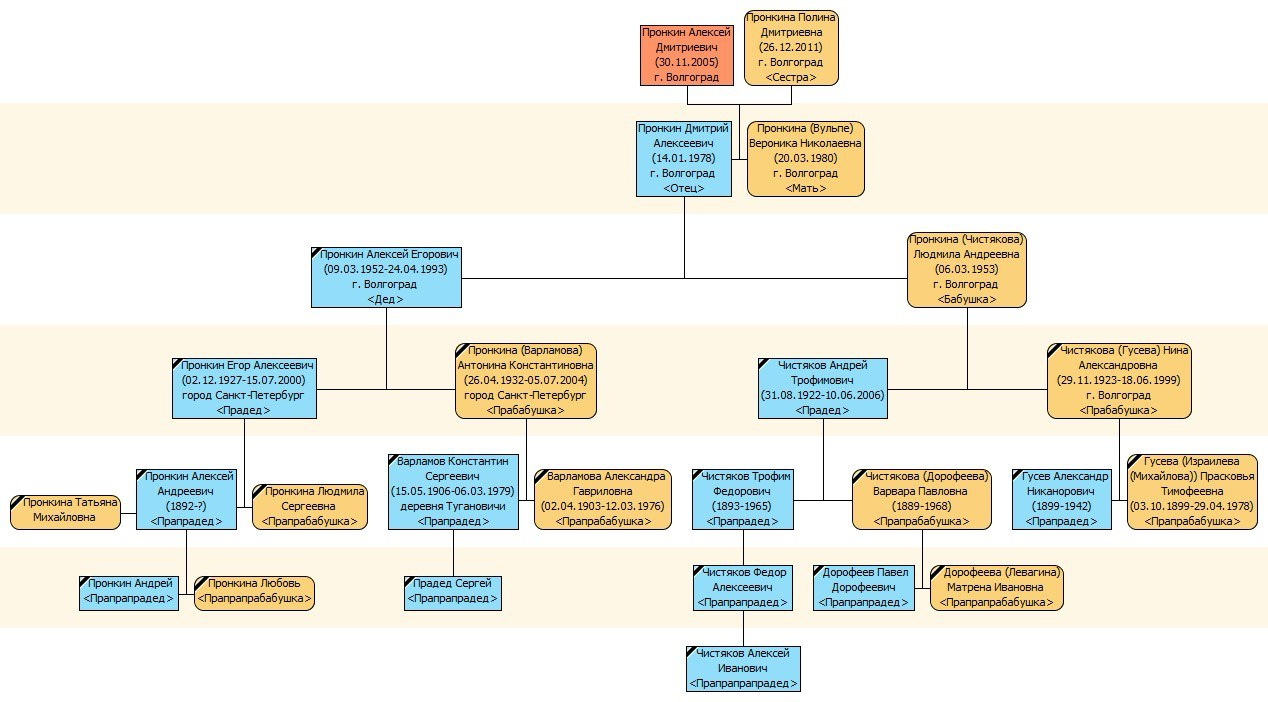
\includegraphics[width=0.8\textwidth]{img/family_tree.jpg}
\end{figure}

% =========================================================
%              Список фактов с описанием аргументов, Список правил с комментариями
% =========================================================
\section*{Список фактов с описанием аргументов и список правил с комментариями}

% \inputminted[linenos, fontsize=\footnotesize]{prolog}{../family2.pl}

% =========================================================
%              Список фактов с описанием аргументов, Список правил с комментариями
% =========================================================
\section*{Результаты выполнения запросов}

% \begin{figure}[h!]
%   % 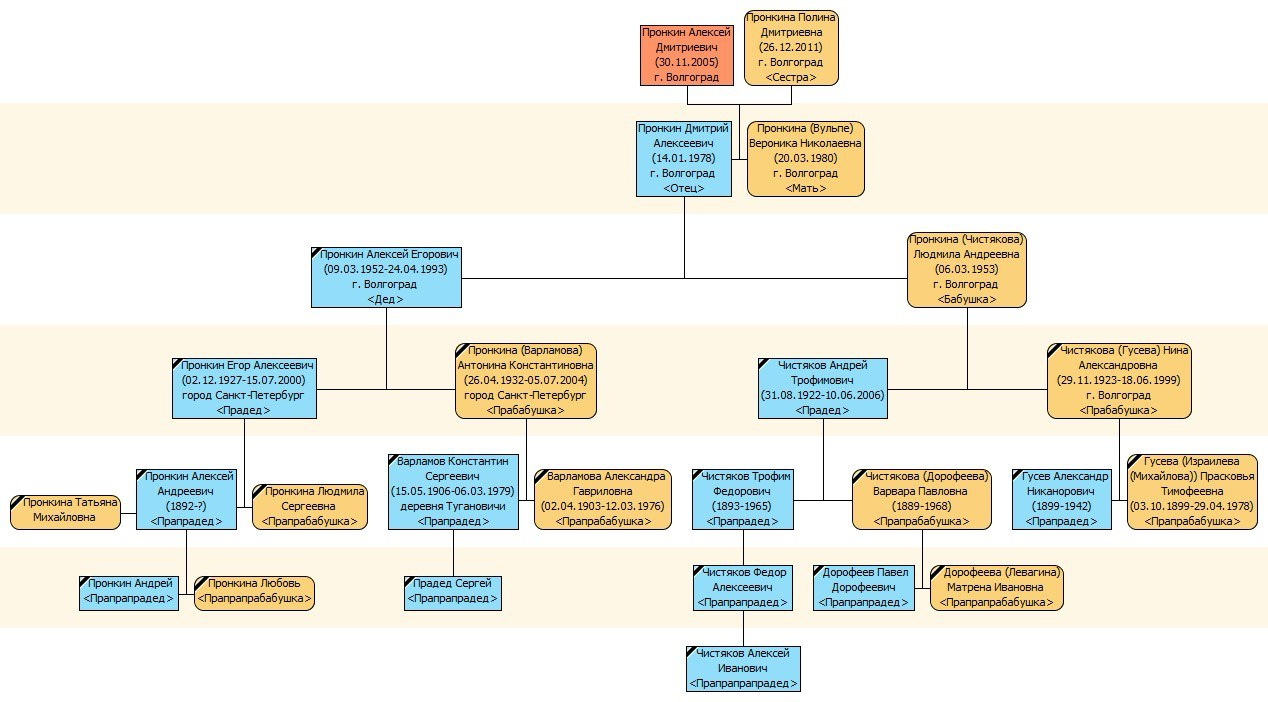
\includegraphics[width=0.8\textwidth]{img/family_tree.jpg}
% \end{figure}

\end{document}
